% Content below is autogenerated 
\subsection{Technical details on low-power jammer 'S1.1'}
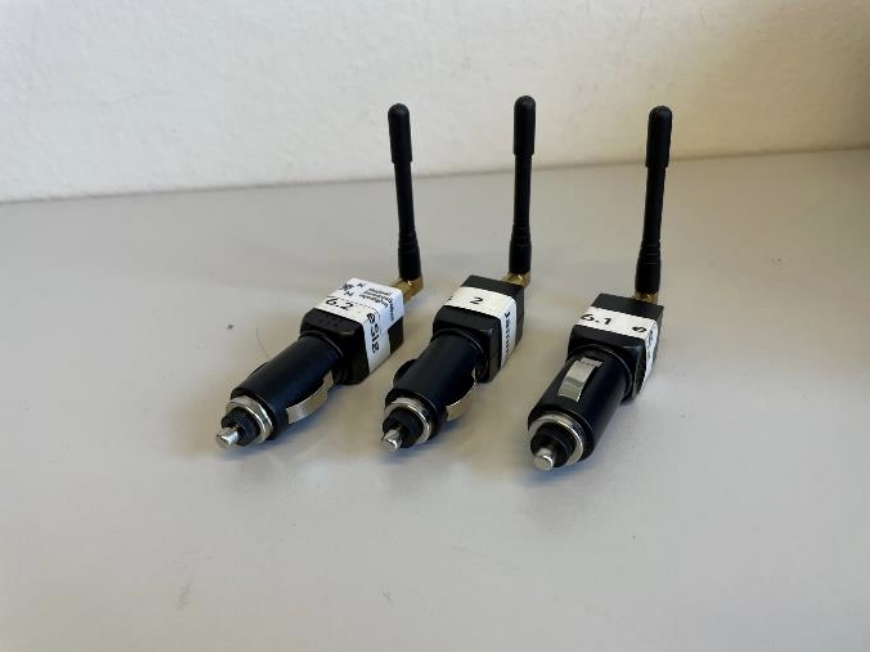
\includegraphics[scale=0.4]{../graphics/appendixG/s1.1-photo.png}\\ \\ 
The jammer S1.1 belongs to the 'Cigarette jammer' category of jammers. Such jammers are often installed in the cigarette lighter outlet in cars. They are intended to cover the car, and a given radius around the car. \\S1.1 is an one-antenna, so-called 'L1-only', jammer, disrupting only the upper L-band.\\
\begin{table}[H]\centering
\begin{tabular}{|c|c|c|c|c|c|c|}\rowcolor[HTML]{C0C0C0} 
\hline
\makecell{Centre frequency\\{[MHz]}} & \makecell{Bandwidth\\{[MHz]}} & \makecell{PSD\\{[dBm/MHz]}} & \makecell{TX total\\{[dBm]}} & \makecell{CF max\\{[dBm]}} & \makecell{Sweep rate\\{[µs]}} & \makecell{Modulation}\\ 
\hline
\makecell{1577.40} & \makecell{29.96} & \makecell{7.58} & \makecell{22.34} & \makecell{7.89} & \makecell{37.1} & \makecell{Sawtooth}\\ 
\hline\end{tabular}\caption{Technical characteristics of S1.1 jammer}\label{table:tech_char_S1.1}\end{table}
